\documentclass[12pt]{article}
\usepackage[a4paper, total={7in, 10in}]{geometry}
\usepackage{amsmath}
\usepackage{graphicx}
\usepackage{multicol}
\usepackage{amssymb}
\usepackage{tabularx}
\setlength{\parindent}{0pt}

\title{Complex Numbers (Part 1) Lesson\vspace{-3mm}}
\author{2018-2019 SLSS Math Club\vspace{-5mm}}
\date{April 10, 2019\vspace{-5mm}}

\begin{document}
\maketitle

\section{Introduction}
A complex number is a number which can be written in the form $z=a + bi$, where $a$ and $b$ are real numbers and $i$ is the imaginary unit defined as $i = \sqrt{-1}$. The set of complex numbers is usually denoted by the mathematical symbol $\mathbb{C}$. Some examples of complex numbers are shown below:
\begin{align*}
    5 - 4i && -2i && -3 + 6i && 10
\end{align*}

\section{Complex Number Arithmetic}
As stated earlier $i$ is defined as $i = \sqrt{-1}$. Some important properties which may be useful are:
\begin{align*}
    i = \sqrt{-1} && i^2 = -1 && i^3 = -i && i^4 = 1
\end{align*}

\textbf{Example:} Simplify $i^{2018}$
\begin{align*}
    i^{2018} &= i^{2016 + 2} \\
            &= i^{4(54) + 2} \\
            &= (1)(i^2) \\
            &= -1
\end{align*}

\subsection{Addition and Subtraction}
Adding and subtracting complex numbers follows the same principle of adding and subtracting like terms. The real parts of complex numbers are considered to be like terms and the imaginary parts are considered to be like terms. \\

\textbf{Example:} Simplify $(4 + 3i) + (2 - i)$
\begin{align*}
    (4 + 3i) + (2 - i) &= 4 + 3i + 2 - i \\
    &= 6 + 2i
\end{align*}

\subsection{Multiplication}
Multiplying complex numbers follows the same principle of multiplying binomials. The main difference is that when two imaginary numbers are multiplied, the product is a real number. \\

\textbf{Example:} Simplify $(3 + 2i)(4 - 2i)$
\begin{align*}
    (3 + 2i)(4 - 2i) &= 12 - 6i + 8i - 4i^2 \\
    &= 12 + 2i -4(-1) \\
    &= 16 + 2i
\end{align*}

\subsection{Complex Conjugate}
The complex conjugate of a complex number $a + bi$ is $a - bi$. The following are complex conjugates:
\begin{align*}
    -5 + 6i \text{ and } -5 -6i && -2i \text{ and } 2i && 17 \text{ and } 17
\end{align*}

Complex conjugates are often used for rationalizing denominators that contain complex numbers. \\

\textbf{Example:} Rationalize $\displaystyle{\frac{3 + 2i}{5 - 2i}}$
\begin{align*}
    \frac{3 + 2i}{5 - 2i} &= \frac{(3 + 2i)(5 + 2i)}{(5 - 2i)(5 + 2i)} \\
    &= \frac{11 + 16i}{29} \\
    &= \frac{11}{29} + \frac{16}{29}i
\end{align*}

\section{Complex Plane}
Complex numbers are often represented on a complex plane, also known as the Argand plane. The real axis ($\Re(z)$) corresponds to the $x$-axis and the imaginary axis ($\Im(z)$) corresponds to the $y$-axis. The complex number $a + bi$ is graphed on this plane as the ordered plane $(a, b)$.
\begin{center}
    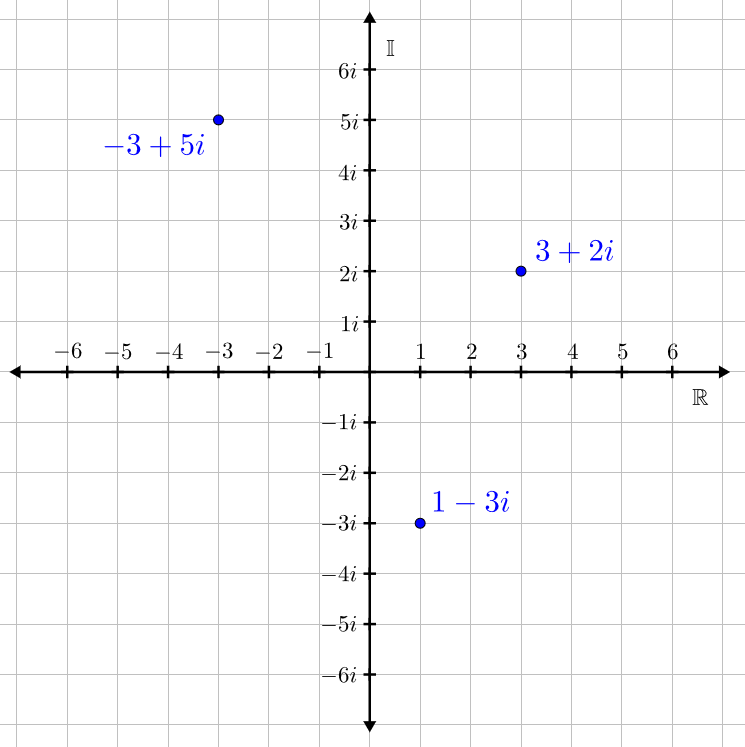
\includegraphics[scale = 0.25]{Graphics/Week_12/ArgandPlane.png}
\end{center}

\subsection{Complex Modulus}
The absolute value, or complex modulus, of a complex number $z=a + bi$ is defined as the positive distance from the origin to the complex number $z$ on the complex plane. It is calculated as $$|z|=|a + bi| = \sqrt{a^2 + b^2}$$

\subsection{Complex Argument}
The complex argument of a complex number $z = a + bi$ is defined as the angle that the positive real axis makes with the terminal arm that connects the origin with the complex number $z$. The angle $\theta$ is calculated as $$\tan{\theta} = \frac{b}{a}$$ $\theta$ can be solved for by taking the inverse tangent of the above equation, however, it is important to account for the quadrant that the complex number is located in.

\end{document}